\documentclass[UTF8]{ctexart}
\usepackage[a4paper,margin=1.8cm]{geometry}
\usepackage{graphicx}
\usepackage{float}
\usepackage{longtable}
\usepackage{array}
\usepackage{xcolor}
\usepackage{fancyvrb}
\usepackage{hyperref}
\setlength{\parindent}{0pt}
\setlength{\parskip}{0.45em}
\begin{document}
\section*{期末复习 PPT 完整模拟卷 02（题目与完整解析）}

\subsection*{卷面说明}

\begin{Verbatim}[fontsize=\small,breaklines=true]
考试时间：150 分钟
总分：100 分
题型：计算、构造、翻译与简答
说明：本卷题面给出了全部文法、控制流、数据流和目标机条件，不需要查阅其他文件。
\end{Verbatim}

\subsection*{A 卷题目}

\subsubsection*{一、词法分析与 LL(1) 分析（20 分）}

\paragraph*{（一）词法分析（10 分）}

给定正则表达式：

\begin{Verbatim}[fontsize=\small,breaklines=true]
(a|b)*a
\end{Verbatim}

1. 使用 Thompson 构造法构造等价 NFA，写出起始状态、接受状态和全部转移。 2. 使用子集构造法构造 DFA，写出每个 DFA 状态对应的 NFA 状态集合及转移表。 3. 最小化 DFA，写出最终状态集合和转移表。

\paragraph*{（二）LL(1) 分析（10 分）}

给定文法，\texttt{p、r、t、u} 均为终结符：

\begin{Verbatim}[fontsize=\small,breaklines=true]
A -> B C
B -> B p | r
C -> t | u
\end{Verbatim}

1. 消除直接左递归。 2. 计算所有非终结符的 FIRST 和 FOLLOW。 3. 构造预测分析表。 4. 判断改写后的文法是否为 LL(1)，并写出依据。

\subsubsection*{二、LR 分析与语义分析（20 分）}

\paragraph*{（一）SLR 分析（12 分）}

给定增广文法：

\begin{Verbatim}[fontsize=\small,breaklines=true]
(0) S' -> S
(1) S  -> C C
(2) C  -> c C
(3) C  -> d
\end{Verbatim}

1. 构造完整规范 LR(0) 项集族，并写出全部 GOTO 转移。 2. 计算 FOLLOW(S) 和 FOLLOW(C)。 3. 构造完整 SLR ACTION/GOTO 表。 4. 判断是否存在移进-规约或规约-规约冲突。

\paragraph*{（二）L 属性 SDD（8 分）}

给定声明文法：

\begin{Verbatim}[fontsize=\small,breaklines=true]
D  -> T L
T  -> int | float
L  -> id L'
L' -> , id L' | epsilon
\end{Verbatim}

设计一个 L 属性 SDD，将每个 \texttt{id} 及其类型加入符号表；再写出分析输入 \texttt{float x, y} 时的属性传递顺序和最终符号表。

\subsubsection*{三、中间代码、控制流与 SSA（20 分）}

给定程序片段，假定数组元素宽度为 4：

\begin{Verbatim}[fontsize=\small,breaklines=true]
while (i < n) {
    if (a[i] > 0)
        sum = sum + a[i];
    i = i + 1;
}
\end{Verbatim}

1. 生成完整三地址码，要求显式写出标签和跳转目标。 2. 划分基本块并写出 CFG 边。 3. 把程序改写成 SSA，要求正确放置 \texttt{i} 和 \texttt{sum} 的 phi 函数。 4. 说明两个 phi 函数在退出 SSA 时应在哪些控制流边上插入复制。

\subsubsection*{四、运行时环境与目标代码生成（20 分）}

\paragraph*{（一）运行时环境（10 分）}

函数调用如下：

\begin{Verbatim}[fontsize=\small,breaklines=true]
int add(int a, int b) {
    int t = a + b;
    return t;
}

int main() {
    int x = 3;
    int y = 4;
    int z = add(x, y);
    return z;
}
\end{Verbatim}

1. 写出 \texttt{add} 的活动记录中至少应包含的内容。 2. 按“参数从右到左压栈”的约定，写出调用 \texttt{add(x, y)} 时的压栈顺序。 3. 说明 BP、SP、返回地址和返回值在调用/返回过程中的作用。 4. 比较引用计数与标记-清扫回收，指出引用计数无法处理的结构。

\paragraph*{（二）目标代码生成（10 分）}

三地址码如下，目标机只有寄存器 \texttt{R0、R1}：

\begin{Verbatim}[fontsize=\small,breaklines=true]
t1 = a - b
t2 = t1 + c
x  = t2
\end{Verbatim}

目标机指令为：

\begin{Verbatim}[fontsize=\small,breaklines=true]
LD R, x
ST x, R
ADD Rd, Rs
SUB Rd, Rs
\end{Verbatim}

其中 \texttt{ADD Rd, Rs} 表示 \texttt{Rd = Rd + Rs}，\texttt{SUB Rd, Rs} 表示 \texttt{Rd = Rd - Rs}。

1. 生成一组完整目标代码。 2. 逐条写出寄存器描述符变化。 3. 写出最终地址描述符中 \texttt{x} 的位置。

\subsubsection*{五、数据流分析、支配与自然循环（20 分）}

CFG 和基本块定值如下：

\begin{Verbatim}[fontsize=\small,breaklines=true]
Entry -> B1
B1 -> B2
B2 -> B3
B2 -> B4
B3 -> B2
B4 -> Exit

B1:
  d1: x = 1
  d2: y = 2

B2:
  d3: z = x + y

B3:
  d4: x = z

B4:
  use(z)
\end{Verbatim}

1. 写出到达定值分析的方向、交汇运算和传递方程。 2. 写出每个基本块的 gen/kill。 3. 从空集初始化，计算各基本块最终 IN/OUT。 4. 计算各基本块的支配集合和直接支配者。 5. 找出回边，并写出对应自然循环。

\subsection*{B 按考试标准重写答案}

\subsubsection*{一、词法分析与 LL(1) 分析答案}

\paragraph*{（一）词法分析}

正则表达式是：

\begin{Verbatim}[fontsize=\small,breaklines=true]
(a|b)*a
\end{Verbatim}

它表示任意个 \texttt{a} 或 \texttt{b} 后面再接一个 \texttt{a}，也就是所有以 \texttt{a} 结尾的 \texttt{\textbackslash{}\{a,b\textbackslash{}\}} 串。

Thompson NFA 如图。起始状态为 \texttt{q0}，接受状态为 \texttt{q9}。

\begin{figure}[H]\centering
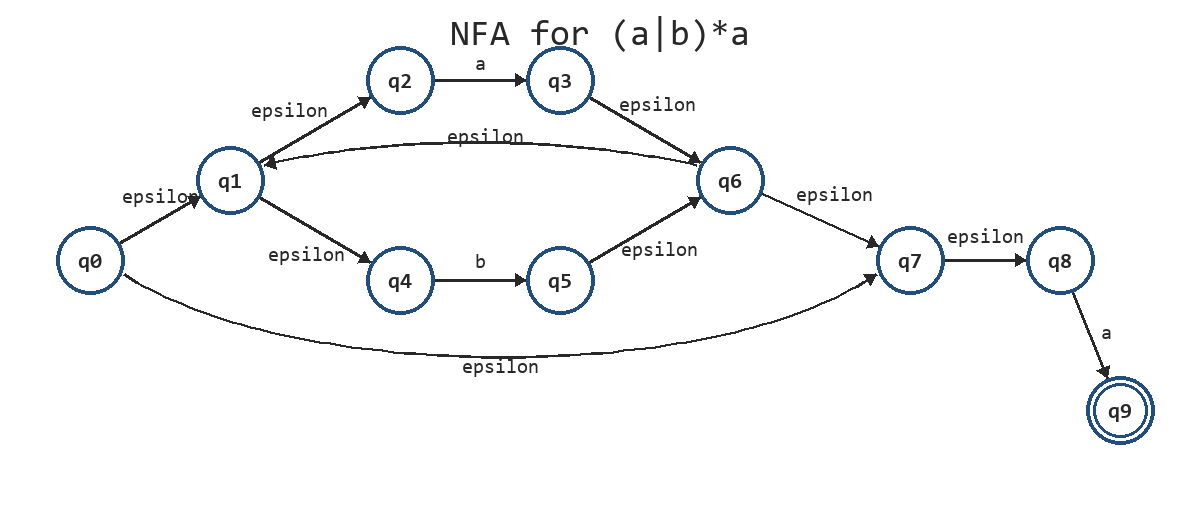
\includegraphics[width=0.82\linewidth]{figures/nfa-thompson-abstar-a.png}
\par{\small Thompson NFA for (a|b)*a}
\end{figure}

NFA 转移表：

\begin{longtable}{|p{0.19\linewidth}|p{0.19\linewidth}|p{0.19\linewidth}|p{0.19\linewidth}|p{0.19\linewidth}|}
\hline
起点 & 边标号 & 终点 & 含义 &  \\
\hline
\endfirsthead
起点 & 边标号 & 终点 & 含义 &  \\
\hline
\endhead
q0 & epsilon & q1 & 进入 `(a & b)*` \\
\hline
q0 & epsilon & q7 & \texttt{*} 重复 0 次 &  \\
\hline
q1 & epsilon & q2 & 选择 \texttt{a} 分支 &  \\
\hline
q1 & epsilon & q4 & 选择 \texttt{b} 分支 &  \\
\hline
q2 & a & q3 & 匹配 \texttt{a} &  \\
\hline
q4 & b & q5 & 匹配 \texttt{b} &  \\
\hline
q3 & epsilon & q6 & 分支结束 &  \\
\hline
q5 & epsilon & q6 & 分支结束 &  \\
\hline
q6 & epsilon & q1 & \texttt{*} 回到循环 &  \\
\hline
q6 & epsilon & q7 & \texttt{*} 退出循环 &  \\
\hline
q7 & epsilon & q8 & 连接最后一个 \texttt{a} &  \\
\hline
q8 & a & q9 & 匹配末尾 \texttt{a} &  \\
\hline
\end{longtable}

子集构造从初态闭包开始：

\begin{Verbatim}[fontsize=\small,breaklines=true]
D0 = epsilon-closure({q0}) = {q0,q1,q2,q4,q7,q8}
\end{Verbatim}

逐步计算：

\begin{longtable}{|p{0.19\linewidth}|p{0.19\linewidth}|p{0.19\linewidth}|p{0.19\linewidth}|p{0.19\linewidth}|}
\hline
DFA 状态 & NFA 状态集合 & 输入 a 后 & 输入 b 后 & 是否接受 \\
\hline
\endfirsthead
DFA 状态 & NFA 状态集合 & 输入 a 后 & 输入 b 后 & 是否接受 \\
\hline
\endhead
D0 & \texttt{\textbackslash{}\{q0,q1,q2,q4,q7,q8\textbackslash{}\}} & D1 & D2 & 否 \\
\hline
D1 & \texttt{\textbackslash{}\{q1,q2,q3,q4,q6,q7,q8,q9\textbackslash{}\}} & D1 & D2 & 是 \\
\hline
D2 & \texttt{\textbackslash{}\{q1,q2,q4,q5,q6,q7,q8\textbackslash{}\}} & D1 & D2 & 否 \\
\hline
\end{longtable}

接受状态判断依据：NFA 状态集合中包含 \texttt{q9}。因此只有 \texttt{D1} 是 DFA 接受状态。

\begin{figure}[H]\centering
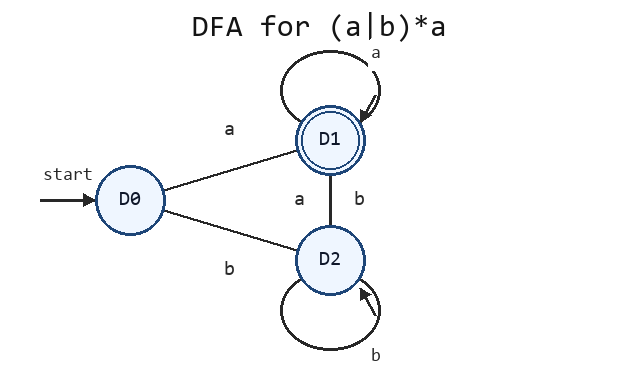
\includegraphics[width=0.82\linewidth]{figures/dfa-subset-abstar-a.png}
\par{\small 子集构造 DFA for (a|b)*a}
\end{figure}

最小化时先按终态与非终态分组：

\begin{Verbatim}[fontsize=\small,breaklines=true]
P0 = { {D1}, {D0,D2} }
\end{Verbatim}

比较 \texttt{D0} 和 \texttt{D2}：

\begin{longtable}{|p{0.23\linewidth}|p{0.23\linewidth}|p{0.23\linewidth}|p{0.23\linewidth}|}
\hline
状态 & 输入 a & 输入 b & 结论 \\
\hline
\endfirsthead
状态 & 输入 a & 输入 b & 结论 \\
\hline
\endhead
D0 & D1 & D2 & a 到终态组，b 到非终态组 \\
\hline
D2 & D1 & D2 & a 到终态组，b 到非终态组 \\
\hline
\end{longtable}

\texttt{D0} 和 \texttt{D2} 对所有输入都转到相同分组，所以等价，可以合并。令：

\begin{Verbatim}[fontsize=\small,breaklines=true]
N = {D0,D2}
F = {D1}
\end{Verbatim}

最小 DFA：

\begin{longtable}{|p{0.23\linewidth}|p{0.23\linewidth}|p{0.23\linewidth}|p{0.23\linewidth}|}
\hline
最小状态 & 输入 a & 输入 b & 是否接受 \\
\hline
\endfirsthead
最小状态 & 输入 a & 输入 b & 是否接受 \\
\hline
\endhead
N & F & N & 否 \\
\hline
F & F & N & 是 \\
\hline
\end{longtable}

\begin{figure}[H]\centering
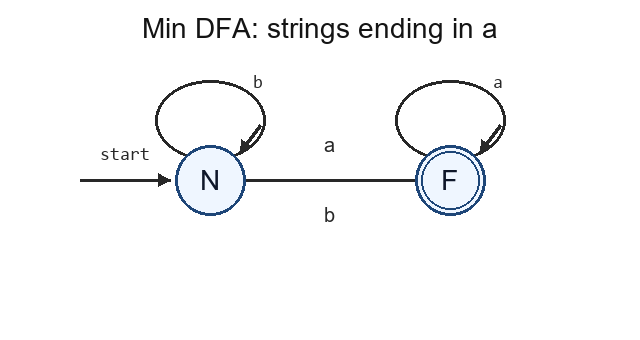
\includegraphics[width=0.82\linewidth]{figures/dfa-min-abstar-a.png}
\par{\small 最小 DFA for (a|b)*a}
\end{figure}

\paragraph*{（二）LL(1) 分析}

原文法：

\begin{Verbatim}[fontsize=\small,breaklines=true]
A -> B C
B -> B p | r
C -> t | u
\end{Verbatim}

\texttt{B -> B p | r} 是直接左递归。套用：

\begin{Verbatim}[fontsize=\small,breaklines=true]
X  -> X alpha | beta
X  -> beta X'
X' -> alpha X' | epsilon
\end{Verbatim}

其中 \texttt{alpha=p}，\texttt{beta=r}，得到：

\begin{Verbatim}[fontsize=\small,breaklines=true]
A  -> B C
B  -> r B'
B' -> p B' | epsilon
C  -> t | u
\end{Verbatim}

FIRST 集：

\begin{longtable}{|p{0.23\linewidth}|p{0.23\linewidth}|p{0.23\linewidth}|p{0.23\linewidth}|}
\hline
非终结符 & 推导依据 & FIRST &  \\
\hline
\endfirsthead
非终结符 & 推导依据 & FIRST &  \\
\hline
\endhead
B & \texttt{B -> r B'} & \texttt{\textbackslash{}\{ r \textbackslash{}\}} &  \\
\hline
B' & `B' -> p B' & epsilon` & \texttt{\textbackslash{}\{ p, epsilon \textbackslash{}\}} \\
\hline
C & `C -> t & u` & \texttt{\textbackslash{}\{ t, u \textbackslash{}\}} \\
\hline
A & \texttt{A -> B C}，B 不能推出 epsilon & \texttt{\textbackslash{}\{ r \textbackslash{}\}} &  \\
\hline
\end{longtable}

FOLLOW 集：

\begin{longtable}{|p{0.31\linewidth}|p{0.31\linewidth}|p{0.31\linewidth}|}
\hline
FOLLOW 集 & 推导依据 & 结果 \\
\hline
\endfirsthead
FOLLOW 集 & 推导依据 & 结果 \\
\hline
\endhead
FOLLOW(A) & A 是开始符号 & \texttt{\textbackslash{}\{ \textbackslash{}\$ \textbackslash{}\}} \\
\hline
FOLLOW(B) & \texttt{A -> B C}，B 后面是 C & \texttt{\textbackslash{}\{ t, u \textbackslash{}\}} \\
\hline
FOLLOW(B') & \texttt{B -> r B'}，B' 在末尾 & \texttt{\textbackslash{}\{ t, u \textbackslash{}\}} \\
\hline
FOLLOW(C) & \texttt{A -> B C}，C 在末尾 & \texttt{\textbackslash{}\{ \textbackslash{}\$ \textbackslash{}\}} \\
\hline
\end{longtable}

预测分析表填表依据：

\begin{longtable}{|p{0.31\linewidth}|p{0.31\linewidth}|p{0.31\linewidth}|}
\hline
产生式 & 依据 & 表项 \\
\hline
\endfirsthead
产生式 & 依据 & 表项 \\
\hline
\endhead
\texttt{A -> B C} & FIRST(BC)=\{r\} & \texttt{M[A,r]} \\
\hline
\texttt{B -> r B'} & FIRST(rB')=\{r\} & \texttt{M[B,r]} \\
\hline
\texttt{B' -> p B'} & FIRST(pB')=\{p\} & \texttt{M[B',p]} \\
\hline
\texttt{B' -> epsilon} & FOLLOW(B')=\{t,u\} & \texttt{M[B',t]}，\texttt{M[B',u]} \\
\hline
\texttt{C -> t} & FIRST(t)=\{t\} & \texttt{M[C,t]} \\
\hline
\texttt{C -> u} & FIRST(u)=\{u\} & \texttt{M[C,u]} \\
\hline
\end{longtable}

完整预测分析表，空白处为 error：

\begin{longtable}{|p{0.16\linewidth}|p{0.16\linewidth}|p{0.16\linewidth}|p{0.16\linewidth}|p{0.16\linewidth}|p{0.16\linewidth}|}
\hline
非终结符 & r & p & t & u & \$ \\
\hline
\endfirsthead
非终结符 & r & p & t & u & \$ \\
\hline
\endhead
A & \texttt{A -> B C} & error & error & error & error \\
\hline
B & \texttt{B -> r B'} & error & error & error & error \\
\hline
B' & error & \texttt{B' -> p B'} & \texttt{B' -> epsilon} & \texttt{B' -> epsilon} & error \\
\hline
C & error & error & \texttt{C -> t} & \texttt{C -> u} & error \\
\hline
\end{longtable}

每个表项最多一条产生式，因此改写后的文法是 LL(1)。

\subsubsection*{二、LR 分析与语义分析答案}

\paragraph*{（一）SLR 分析}

增广文法：

\begin{Verbatim}[fontsize=\small,breaklines=true]
(0) S' -> S
(1) S  -> C C
(2) C  -> c C
(3) C  -> d
\end{Verbatim}

规范 LR(0) 项集族：

\begin{Verbatim}[fontsize=\small,breaklines=true]
I0:
S' -> . S
S  -> . C C
C  -> . c C
C  -> . d

I1:
S' -> S .

I2:
S  -> C . C
C  -> . c C
C  -> . d

I3:
C  -> c . C
C  -> . c C
C  -> . d

I4:
C  -> d .

I5:
S  -> C C .

I6:
C  -> c C .
\end{Verbatim}

GOTO 转移表：

\begin{longtable}{|p{0.31\linewidth}|p{0.31\linewidth}|p{0.31\linewidth}|}
\hline
来源 & 符号 & 目标 \\
\hline
\endfirsthead
来源 & 符号 & 目标 \\
\hline
\endhead
I0 & S & I1 \\
\hline
I0 & C & I2 \\
\hline
I0 & c & I3 \\
\hline
I0 & d & I4 \\
\hline
I2 & C & I5 \\
\hline
I2 & c & I3 \\
\hline
I2 & d & I4 \\
\hline
I3 & C & I6 \\
\hline
I3 & c & I3 \\
\hline
I3 & d & I4 \\
\hline
\end{longtable}

FOLLOW：

\begin{longtable}{|p{0.31\linewidth}|p{0.31\linewidth}|p{0.31\linewidth}|}
\hline
非终结符 & 推导依据 & FOLLOW \\
\hline
\endfirsthead
非终结符 & 推导依据 & FOLLOW \\
\hline
\endhead
S & S 是开始符号 & \texttt{\textbackslash{}\{ \textbackslash{}\$ \textbackslash{}\}} \\
\hline
C & \texttt{S -> C C}：第一个 C 后接 C，加入 FIRST(C)=\{c,d\}；第二个 C 在末尾，加入 FOLLOW(S) & \texttt{\textbackslash{}\{ c,d,\textbackslash{}\$ \textbackslash{}\}} \\
\hline
\end{longtable}

SLR 填表规则：

\begin{Verbatim}[fontsize=\small,breaklines=true]
点前进到终结符时填 shift。
完成项 A -> alpha . 只在 FOLLOW(A) 上填 reduce。
S' -> S . 在 $ 上填 acc。
\end{Verbatim}

完整 SLR ACTION/GOTO 表：

\begin{longtable}{|p{0.16\linewidth}|p{0.16\linewidth}|p{0.16\linewidth}|p{0.16\linewidth}|p{0.16\linewidth}|p{0.16\linewidth}|}
\hline
状态 & ACTION(c) & ACTION(d) & ACTION(\$) & GOTO(S) & GOTO(C) \\
\hline
\endfirsthead
状态 & ACTION(c) & ACTION(d) & ACTION(\$) & GOTO(S) & GOTO(C) \\
\hline
\endhead
0 & s3 & s4 & error & 1 & 2 \\
\hline
1 & error & error & acc & error & error \\
\hline
2 & s3 & s4 & error & error & 5 \\
\hline
3 & s3 & s4 & error & error & 6 \\
\hline
4 & r3 & r3 & r3 & error & error \\
\hline
5 & error & error & r1 & error & error \\
\hline
6 & r2 & r2 & r2 & error & error \\
\hline
\end{longtable}

冲突判断：表中没有任何单元格同时出现 shift 和 reduce，也没有任何单元格同时出现两个 reduce，所以不存在移进-规约冲突或规约-规约冲突。

\paragraph*{（二）L 属性 SDD}

设计思路：\texttt{T.type} 是类型来源，向右传给 \texttt{L.in} 和 \texttt{L'.in}，每遇到一个 \texttt{id} 就把该名字和传入类型加入符号表。

\begin{longtable}{|p{0.47\linewidth}|p{0.47\linewidth}|}
\hline
产生式 & 语义规则或动作 \\
\hline
\endfirsthead
产生式 & 语义规则或动作 \\
\hline
\endhead
\texttt{D -> T L} & \texttt{L.in = T.type} \\
\hline
\texttt{T -> int} & \texttt{T.type = int} \\
\hline
\texttt{T -> float} & \texttt{T.type = float} \\
\hline
\texttt{L -> id L'} & \texttt{addType(id.name, L.in)}；\texttt{L'.in = L.in} \\
\hline
\texttt{L' -> , id L'1} & \texttt{addType(id.name, L'.in)}；\texttt{L'1.in = L'.in} \\
\hline
\texttt{L' -> epsilon} & 不执行插入动作 \\
\hline
\end{longtable}

输入 \texttt{float x, y} 的属性传递：

\begin{longtable}{|p{0.31\linewidth}|p{0.31\linewidth}|p{0.31\linewidth}|}
\hline
步骤 & 动作 & 结果 \\
\hline
\endfirsthead
步骤 & 动作 & 结果 \\
\hline
\endhead
1 & \texttt{T -> float} & \texttt{T.type=float} \\
\hline
2 & \texttt{D -> T L} & \texttt{L.in=float} \\
\hline
3 & 识别 \texttt{x} & \texttt{addType(x,float)} \\
\hline
4 & 进入 \texttt{L'} & \texttt{L'.in=float} \\
\hline
5 & 识别 \texttt{y} & \texttt{addType(y,float)} \\
\hline
\end{longtable}

最终符号表：

\begin{longtable}{|p{0.47\linewidth}|p{0.47\linewidth}|}
\hline
名字 & 类型 \\
\hline
\endfirsthead
名字 & 类型 \\
\hline
\endhead
x & float \\
\hline
y & float \\
\hline
\end{longtable}

继承属性只依赖父结点或左侧兄弟结点，因此满足 L 属性限制。

\subsubsection*{三、中间代码、控制流与 SSA 答案}

\paragraph*{1. 三地址码}

数组元素宽度为 4，\texttt{a[i]} 的地址偏移为 \texttt{i * 4}。

\begin{Verbatim}[fontsize=\small,breaklines=true]
L1:
if i < n goto L2
goto L6

L2:
t1 = i * 4
t2 = a[t1]
if t2 > 0 goto L3
goto L4

L3:
sum = sum + t2
goto L4

L4:
i = i + 1
goto L1

L6:
\end{Verbatim}

\paragraph*{2. 基本块与 CFG}

\begin{figure}[H]\centering
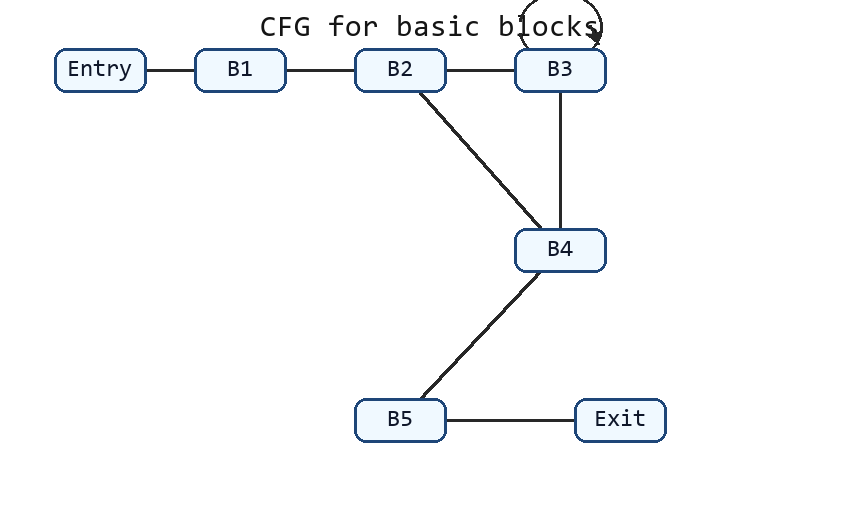
\includegraphics[width=0.82\linewidth]{figures/cfg-09-basic-blocks.png}
\par{\small 基本块 CFG}
\end{figure}

\begin{longtable}{|p{0.47\linewidth}|p{0.47\linewidth}|}
\hline
基本块 & 语句 \\
\hline
\endfirsthead
基本块 & 语句 \\
\hline
\endhead
B1 & \texttt{L1} 条件判断，真到 B2，假到 B5 \\
\hline
B2 & 数组地址计算、读取和 \texttt{a[i] > 0} 判断 \\
\hline
B3 & \texttt{sum = sum + t2} \\
\hline
B4 & \texttt{i = i + 1}，回到 B1 \\
\hline
B5 & \texttt{L6} 循环出口 \\
\hline
\end{longtable}

CFG 边：

\begin{Verbatim}[fontsize=\small,breaklines=true]
B1 -> B2
B1 -> B5
B2 -> B3
B2 -> B4
B3 -> B4
B4 -> B1
\end{Verbatim}

\paragraph*{3. SSA}

循环头 B1 有来自循环外和回边 B4 的两条路径，因此 \texttt{i} 和 \texttt{sum} 都需要 phi。B4 还有来自 B2 假分支和 B3 真分支的汇合，因此 \texttt{sum} 在 B4 也需要 phi。

\begin{Verbatim}[fontsize=\small,breaklines=true]
L1:
i1   = phi(i0, i2)
sum1 = phi(sum0, sum3)
if i1 < n goto L2
goto L6

L2:
t1 = i1 * 4
t2 = a[t1]
if t2 > 0 goto L3
goto L4

L3:
sum2 = sum1 + t2
goto L4

L4:
sum3 = phi(sum1, sum2)
i2 = i1 + 1
goto L1

L6:
\end{Verbatim}

\paragraph*{4. 退出 SSA 的复制边}

phi 展开原则：在每条前驱边上插入对应复制。

\begin{longtable}{|p{0.31\linewidth}|p{0.31\linewidth}|p{0.31\linewidth}|}
\hline
phi & 前驱边 & 插入复制 \\
\hline
\endfirsthead
phi & 前驱边 & 插入复制 \\
\hline
\endhead
\texttt{i1 = phi(i0, i2)} & 循环外 -> L1 & \texttt{i1 = i0} \\
\hline
\texttt{i1 = phi(i0, i2)} & L4 -> L1 & \texttt{i1 = i2} \\
\hline
\texttt{sum1 = phi(sum0, sum3)} & 循环外 -> L1 & \texttt{sum1 = sum0} \\
\hline
\texttt{sum1 = phi(sum0, sum3)} & L4 -> L1 & \texttt{sum1 = sum3} \\
\hline
\texttt{sum3 = phi(sum1, sum2)} & L2 -> L4 & \texttt{sum3 = sum1} \\
\hline
\texttt{sum3 = phi(sum1, sum2)} & L3 -> L4 & \texttt{sum3 = sum2} \\
\hline
\end{longtable}

这些复制在语义上是并行复制；若控制流边不能直接插入指令，需要拆分边。

\subsubsection*{四、运行时环境与目标代码生成答案}

\paragraph*{（一）运行时环境}

\texttt{add} 的活动记录至少包含：

\begin{longtable}{|p{0.47\linewidth}|p{0.47\linewidth}|}
\hline
内容 & 作用 \\
\hline
\endfirsthead
内容 & 作用 \\
\hline
\endhead
参数 \texttt{a}、\texttt{b} & 被调用函数读取实参 \\
\hline
局部变量 \texttt{t} & 保存 \texttt{a+b} 的局部结果 \\
\hline
返回地址 & 指出 \texttt{add} 返回后继续执行的位置 \\
\hline
旧 BP / 控制链 & 返回时恢复调用者活动记录 \\
\hline
保存的寄存器 & 保护调用前的机器状态 \\
\hline
返回值位置 & 按调用约定传回 \texttt{t} \\
\hline
\end{longtable}

参数从右到左压栈，调用 \texttt{add(x,y)} 的顺序是：

\begin{longtable}{|p{0.47\linewidth}|p{0.47\linewidth}|}
\hline
顺序 & 动作 \\
\hline
\endfirsthead
顺序 & 动作 \\
\hline
\endhead
1 & 压入 \texttt{y} 的值，作为形参 \texttt{b} \\
\hline
2 & 压入 \texttt{x} 的值，作为形参 \texttt{a} \\
\hline
3 & 执行 \texttt{call add}，保存返回地址 \\
\hline
4 & 被调函数建立新活动记录 \\
\hline
\end{longtable}

BP、SP、返回地址、返回值作用：

\begin{longtable}{|p{0.47\linewidth}|p{0.47\linewidth}|}
\hline
项 & 作用 \\
\hline
\endfirsthead
项 & 作用 \\
\hline
\endhead
SP & 指向当前栈顶，压栈和退栈会改变 SP \\
\hline
BP & 当前活动记录的稳定基址，用固定偏移访问参数和局部变量 \\
\hline
返回地址 & 被调函数结束后跳回调用点 \\
\hline
返回值 & 放入约定寄存器或栈中约定位置，供调用者读取 \\
\hline
\end{longtable}

垃圾回收比较：

\begin{longtable}{|p{0.31\linewidth}|p{0.31\linewidth}|p{0.31\linewidth}|}
\hline
方法 & 优点 & 缺点 \\
\hline
\endfirsthead
方法 & 优点 & 缺点 \\
\hline
\endhead
引用计数 & 对象计数变为 0 时可立即回收 & 无法回收不可达环 \\
\hline
标记-清扫 & 从根集标记可达对象，能回收不可达环 & 需要遍历堆，可能产生暂停 \\
\hline
\end{longtable}

引用计数无法处理的结构是不可达循环引用，例如两个对象互相引用但已经没有根指向它们。

\paragraph*{（二）目标代码生成}

三地址码：

\begin{Verbatim}[fontsize=\small,breaklines=true]
t1 = a - b
t2 = t1 + c
x  = t2
\end{Verbatim}

目标代码：

\begin{Verbatim}[fontsize=\small,breaklines=true]
LD  R0, a
LD  R1, b
SUB R0, R1
LD  R1, c
ADD R0, R1
ST  x, R0
\end{Verbatim}

寄存器描述符变化：

\begin{longtable}{|p{0.23\linewidth}|p{0.23\linewidth}|p{0.23\linewidth}|p{0.23\linewidth}|}
\hline
步骤 & 指令 & R0 & R1 \\
\hline
\endfirsthead
步骤 & 指令 & R0 & R1 \\
\hline
\endhead
初始 & - & \texttt{\textbackslash{}\{\textbackslash{}\}} & \texttt{\textbackslash{}\{\textbackslash{}\}} \\
\hline
1 & \texttt{LD R0,a} & \texttt{\textbackslash{}\{a\textbackslash{}\}} & \texttt{\textbackslash{}\{\textbackslash{}\}} \\
\hline
2 & \texttt{LD R1,b} & \texttt{\textbackslash{}\{a\textbackslash{}\}} & \texttt{\textbackslash{}\{b\textbackslash{}\}} \\
\hline
3 & \texttt{SUB R0,R1} & \texttt{\textbackslash{}\{t1\textbackslash{}\}} & \texttt{\textbackslash{}\{b\textbackslash{}\}} \\
\hline
4 & \texttt{LD R1,c} & \texttt{\textbackslash{}\{t1\textbackslash{}\}} & \texttt{\textbackslash{}\{c\textbackslash{}\}} \\
\hline
5 & \texttt{ADD R0,R1} & \texttt{\textbackslash{}\{t2\textbackslash{}\}} & \texttt{\textbackslash{}\{c\textbackslash{}\}} \\
\hline
6 & \texttt{ST x,R0} & \texttt{\textbackslash{}\{t2,x\textbackslash{}\}} & \texttt{\textbackslash{}\{c\textbackslash{}\}} \\
\hline
\end{longtable}

最终地址描述符中：

\begin{Verbatim}[fontsize=\small,breaklines=true]
Addr(x) = {内存位置 x, R0}
\end{Verbatim}

\subsubsection*{五、数据流分析、支配与自然循环答案}

\paragraph*{1. 到达定值分析框架}

到达定值是正向 may 分析：

\begin{Verbatim}[fontsize=\small,breaklines=true]
IN[B]  = union OUT[P]，P 是 B 的所有前驱
OUT[B] = gen[B] union (IN[B] - kill[B])
\end{Verbatim}

初始化按题目要求从空集开始。

\paragraph*{2. gen/kill}

所有定义：

\begin{Verbatim}[fontsize=\small,breaklines=true]
d1: x = 1
d2: y = 2
d3: z = x + y
d4: x = z
\end{Verbatim}

\texttt{d1} 和 \texttt{d4} 都定义 \texttt{x}，互相 kill。

\begin{longtable}{|p{0.31\linewidth}|p{0.31\linewidth}|p{0.31\linewidth}|}
\hline
基本块 & gen & kill \\
\hline
\endfirsthead
基本块 & gen & kill \\
\hline
\endhead
B1 & \texttt{\textbackslash{}\{d1,d2\textbackslash{}\}} & \texttt{\textbackslash{}\{d4\textbackslash{}\}} \\
\hline
B2 & \texttt{\textbackslash{}\{d3\textbackslash{}\}} & \texttt{\textbackslash{}\{\textbackslash{}\}} \\
\hline
B3 & \texttt{\textbackslash{}\{d4\textbackslash{}\}} & \texttt{\textbackslash{}\{d1\textbackslash{}\}} \\
\hline
B4 & \texttt{\textbackslash{}\{\textbackslash{}\}} & \texttt{\textbackslash{}\{\textbackslash{}\}} \\
\hline
\end{longtable}

\paragraph*{3. IN/OUT 不动点结果}

\begin{longtable}{|p{0.31\linewidth}|p{0.31\linewidth}|p{0.31\linewidth}|}
\hline
基本块 & IN & OUT \\
\hline
\endfirsthead
基本块 & IN & OUT \\
\hline
\endhead
B1 & \texttt{\textbackslash{}\{\textbackslash{}\}} & \texttt{\textbackslash{}\{d1,d2\textbackslash{}\}} \\
\hline
B2 & \texttt{\textbackslash{}\{d1,d2,d3,d4\textbackslash{}\}} & \texttt{\textbackslash{}\{d1,d2,d3,d4\textbackslash{}\}} \\
\hline
B3 & \texttt{\textbackslash{}\{d1,d2,d3,d4\textbackslash{}\}} & \texttt{\textbackslash{}\{d2,d3,d4\textbackslash{}\}} \\
\hline
B4 & \texttt{\textbackslash{}\{d1,d2,d3,d4\textbackslash{}\}} & \texttt{\textbackslash{}\{d1,d2,d3,d4\textbackslash{}\}} \\
\hline
\end{longtable}

关键推导：

\begin{Verbatim}[fontsize=\small,breaklines=true]
IN[B2] = OUT[B1] union OUT[B3]
       = {d1,d2} union {d2,d3,d4}
       = {d1,d2,d3,d4}
\end{Verbatim}

所以循环回边使 \texttt{d3}、\texttt{d4} 也能到达 B2。

\paragraph*{4. 支配集合和直接支配者}

支配定义：从 Entry 到某节点的每条路径都经过的节点，才支配该节点。

\begin{longtable}{|p{0.47\linewidth}|p{0.47\linewidth}|}
\hline
节点 & Dom \\
\hline
\endfirsthead
节点 & Dom \\
\hline
\endhead
Entry & \texttt{\textbackslash{}\{Entry\textbackslash{}\}} \\
\hline
B1 & \texttt{\textbackslash{}\{Entry,B1\textbackslash{}\}} \\
\hline
B2 & \texttt{\textbackslash{}\{Entry,B1,B2\textbackslash{}\}} \\
\hline
B3 & \texttt{\textbackslash{}\{Entry,B1,B2,B3\textbackslash{}\}} \\
\hline
B4 & \texttt{\textbackslash{}\{Entry,B1,B2,B4\textbackslash{}\}} \\
\hline
Exit & \texttt{\textbackslash{}\{Entry,B1,B2,B4,Exit\textbackslash{}\}} \\
\hline
\end{longtable}

直接支配者：

\begin{longtable}{|p{0.47\linewidth}|p{0.47\linewidth}|}
\hline
节点 & idom \\
\hline
\endfirsthead
节点 & idom \\
\hline
\endhead
B1 & Entry \\
\hline
B2 & B1 \\
\hline
B3 & B2 \\
\hline
B4 & B2 \\
\hline
Exit & B4 \\
\hline
\end{longtable}

\paragraph*{5. 回边与自然循环}

回边判断：若边 \texttt{n -> h} 中 \texttt{h} 支配 \texttt{n}，则该边是回边。

CFG 中：

\begin{Verbatim}[fontsize=\small,breaklines=true]
B3 -> B2
\end{Verbatim}

因为 \texttt{B2} 支配 \texttt{B3}，所以 \texttt{B3 -> B2} 是回边。

自然循环构造：从回边尾 \texttt{B3} 反向追溯前驱，直到回边头 \texttt{B2}，并包含头和尾：

\begin{Verbatim}[fontsize=\small,breaklines=true]
自然循环 = {B2, B3}
\end{Verbatim}
\end{document}
